\documentclass{article}

\title{Product Specification}
\author{Group 5}
\usepackage{outlines}
\usepackage{graphicx}
\graphicspath{{images/}{../diagrams/}}
\date{}

\begin{document}
    \maketitle
    
    \section{Description}
    The chess application will allow the user to play chess against another person locally, or against an AI which will have \\
    three different difficulties; easy, medium and hard. The application will also be able the track the results of the games and \\
    save the skill rating (using the Elo system) of the users and place them on a scoreboard. The AIs will be at a static rating \\
    for each difficulty level.
    
    \section{System Requirements} 
    \subsection{Functional:}
    \begin{outline}
          \1 Users shall be able to play against another human opponent (multiplayer).
          \1 The system shall appoint rankings to the players of the game, which indicates 
             that the winner of a game is awarded points which will have to be calculated.
          \1 The system keeps track of the results for each game played.
          \2 This enables the system to provide an overview of the ranking of the human participants,
             based on on how many games they have won.
          \1 Users shall be able to play against an AI, which will have 3 levels of difficulty:
          \2 Easy
          \2 Medium
          \2 Hard
          \1 Winning against a more intelligent or higher ranked AI should award more points.
     \end{outline}
     
    \subsection{Non-functional:}
    \begin{outline}
          \1 The system shall be made with 2D graphics.
          \2 It must feature a board layout.
          \2 It must feature player statistics.
          \1 The system shall be implemented on top of a open source graphics engine.
          \2 The game shall be implemented in JavaFX.
          \1 The system shall be programmed in such a way that the ruleset (board size etc.) can easily be changed.
          \1 System shall be programmed in Java.
    \end{outline}
    
    \section{User stories}
        USER STORY 1: As a Chess player I want to play against good chess AI’s 
        so I can become better at chess. \\
        
        \noindent
        USER STORY 2: As a pair of friends, we want to play chess together so we
        can spend more time with each other. \\
        
        \noindent
        USER STORY 3: As a user of the chess game I want my available moves to 
        be visualized when I pick a given chess-piece. \\
        
        \noindent
        USER STORY 4: As a beginner level chess player I want to learn to play 
        the game/basic rules of the game so I can play the game without help. \\
        
        \noindent
        USER STORY 5: As a user I want the moves I make to be viewable through 
        the course of a game. \\
        
        \noindent
        USER STORY 6: As a frequent user of the software i want my MMR to be 
        saved/updated after every match so i can show it to my friends. \\
	
	\vspace{30mm}
    \section{Use case diagram}
    Diagram showcasing the major user operations of the chess application. \\ \\
    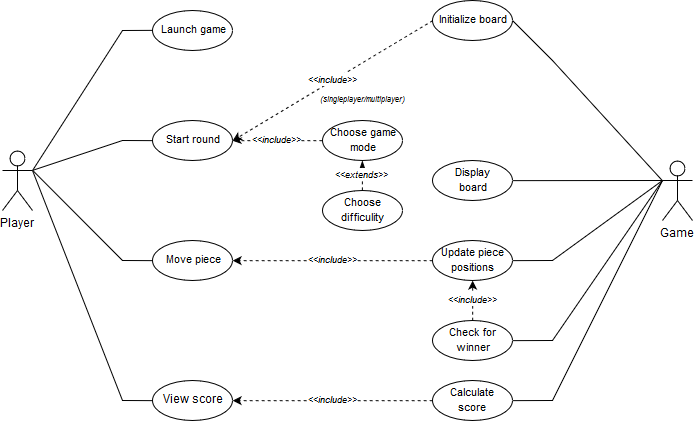
\includegraphics[scale=0.6]{usecase-diagram.png}
    
    \vspace{100mm}
    \section{Use cases}
        \subsection{Use case 1 (fully dressed)}
        A start menu allows a user to start the game and choose single player to
        play against a machine AI. The user will be prompted to write their player
        name so the high score can be saved in an external file. In the next step
        the player has to choose between three difficulties. After the AI difficulty
        is chosen, the game will start. The player must progress by moving their
        pieces according to the game rules. The player can move pieces by clicking
        on their piece (if it is their turn and a legal move) and pick the square that
        the piece should be moved to. The machine will respond according to the 
        difficulty chosen by the player earlier. \\ \\
        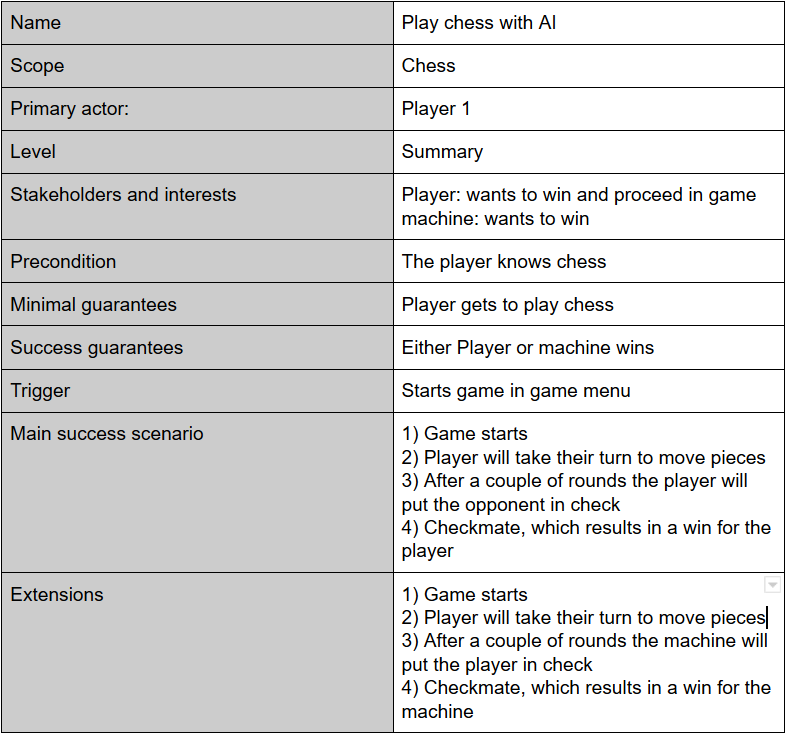
\includegraphics[width=\linewidth]{play-ai.png}
        
        \vspace{30mm}
        \subsection{Use case 2 (fully dressed)}
        A start menu allows a user to start a game and choose multiplayer with 
        another local player. After the player picks the multiplayer option it 
        will be prompted to write name of player 1, then name of player 2, so 
        the high score can be saved in an external file. After the name dialog,
        the players will be taken to the chess game and the possibility to play
        against each other. The game will be started and either player 1 or 2 starts.
        The players must progress with moving their pieces according to the game rules.
        The player can move pieces by clicking on their piece (if it is their 
        turn and a legal move) and pick the square that the piece should be moved
        to. \\ \\
        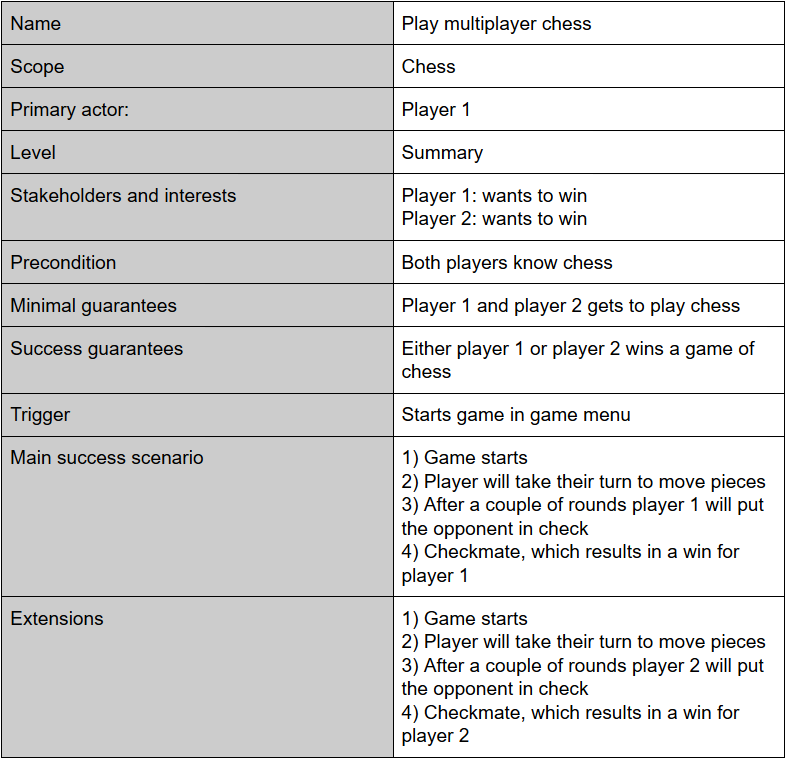
\includegraphics[width=\linewidth]{play-multiplayer.png}
        
    \section{Domain model (class diagram)}
    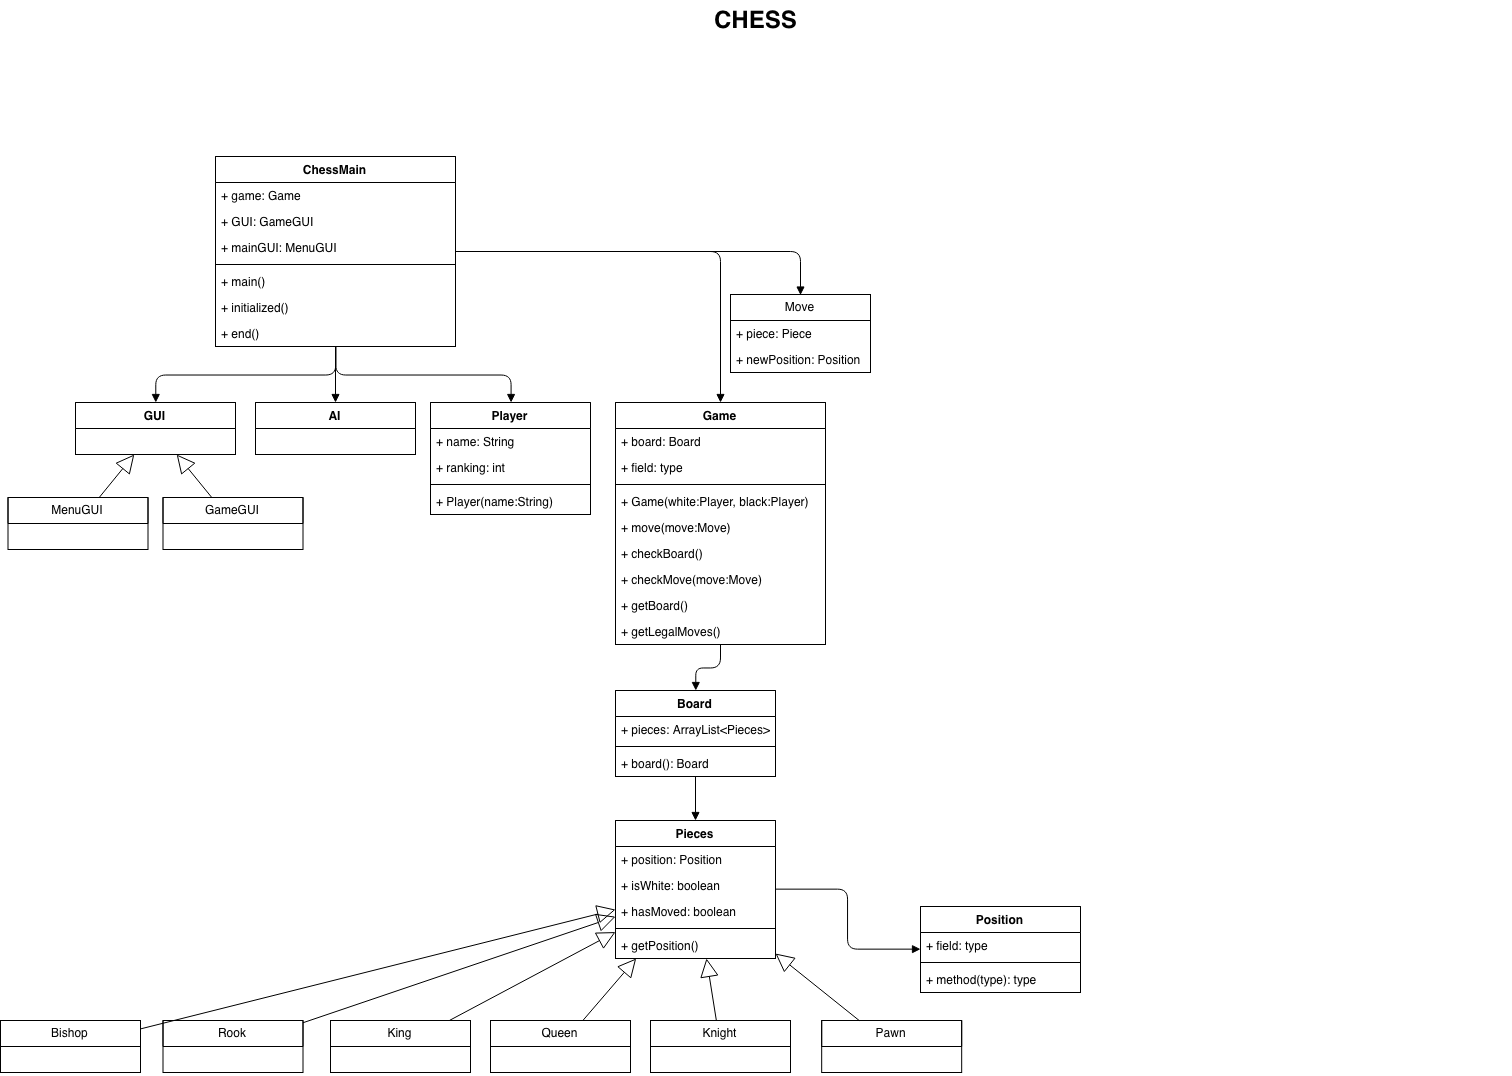
\includegraphics[scale=0.35]{class-diagram.png}
    
    \subsection{Short explanation of the class diagram}
    
        ChessMain:\\
        \begin{outline}
            The ChessMain class is the class where we begin the game (main method).
            \1 main() method will call the initialize(). Once game is initialized we
            will go into an endless loop where we repeatedly asks the GUI/AI for the 
            next move. If the GUI send a resign signal instead of a move we exit the 
            loop and call the end() method. Otherwise we send the move to the game 
            with the game.move() method. This method will return a Boolean value, true means
            everything is ok, and we can go on to the next round. False means that an
            illegal move was made, and we make the GUI tell the player this
            and we let him/her try again until the move is accepted. After a move is made
            we call the game.checkBoard() method. This will check the board after the move
            is made to see if someone has won, there is a check, there is a checkmate or a
            there is a promotion. Here we are only interested in whether someone has won,
            the game will take care of the rest. If someone has won we call the end() method.
            \1 Initialize() method will make a MenuGUI object where the player can 
            provide information about the game he/she is about to play. This information
            is used to initialize a Game and two player objects or one player and one AI object.
            Then we can make a GameGUI object with the game as a parameter.
            \1 end() method will make the GUI display an end screen and calculate
            the new rankings.
        \end{outline}
        
        \noindent
        Game:\\
        \begin{outline}
            The Game class is where we have our current game. It has a board.Board
            variable that is simply a list of all the pieces, the position
            of the pieces is stored in the pieces themselves. The ChessMain class
            will interact with the game via a few methods.
            \1 Move(Piece piece, Position newPos) will simply make a new board.Board
            with updated pieces. This is mostly just a copy of the previous board
            except the piece that were moved and pieces that are knocked out.
            However before we make this new board we have to make sure it’s a
            legal move by calling the checkMove(Piece piece, Position newPos)
            method. If it’s not a legal move it returns false and does nothing,
            otherwise true.
            \1 checkBoard() will check the current board for certain events 
            such as: someone has won, there is a check, there is a checkmate or 
            a there is a promotion. This method will then make a new board if 
            needed. It will return true if someone has won, false otherwise.
            \1 getBoard() the GUI will need the board to display it.
            \1 getLegalMoves(Piece piece) mainly used by the checkMove() method
            but can also be used by the GUI to display legal moves.
        \end{outline}

    
\end{document}
